\clearpage
\section{Results}
\label{sec:results}

\par Table~\ref{table:results} summarizes the expected event yields from signal 
and background. Signal has been scaled by a factor of 100 for visibility. 
Figure~\ref{fig:results} shows the \mt\ distribution for events in the signal region.
The major backgrounds are the exclusive and inclusive WW. 

\begin{table}
\centering
        \resizebox{\textwidth}{!}{
\providecommand{\cutflowTitle}{hsg3}
\begin{tabular}{l||rrr|rr}
Cuts & Inclusive   $WW$ & Exclusive $W^{+}W^{-}$ & Other Bkgs & Total Bkg. & Excl. H [Signal] \\
\hline\hline
\textcolor{blue}{Scale factors} &  & & & & \color{blue}NF = 100.00  \\
$\Delta\phi_{\ell\ell}<1.8$ & 1779.36 $\pm$ 7.96 & 2.31 $\pm$ 0.03 & 6783.23 $\pm$ 227.73 & 8570.49 $\pm$ 227.87 & 2.98 $\pm$ 0.03 \\
$\Delta z^{0}_{ll}<1.0$ & 1776.68 $\pm$ 7.95 & 2.31 $\pm$ 0.03 & 6774.47 $\pm$ 227.72 & 8559.04 $\pm$ 227.86 & 2.98 $\pm$ 0.03 \\
1 mm Exclusive & 0.70 $\pm$ 0.10 & 1.25 $\pm$ 0.02 & 0.10 $\pm$ 0.06 & 2.05 $\pm$ 0.12 & 1.62 $\pm$ 0.02 \\
\end{tabular}
}
\caption{Main contributions to signal region contamination are inclusive WW and exclusive WW}
\label{table:results}
\end{table}

\begin{figure}
\centering
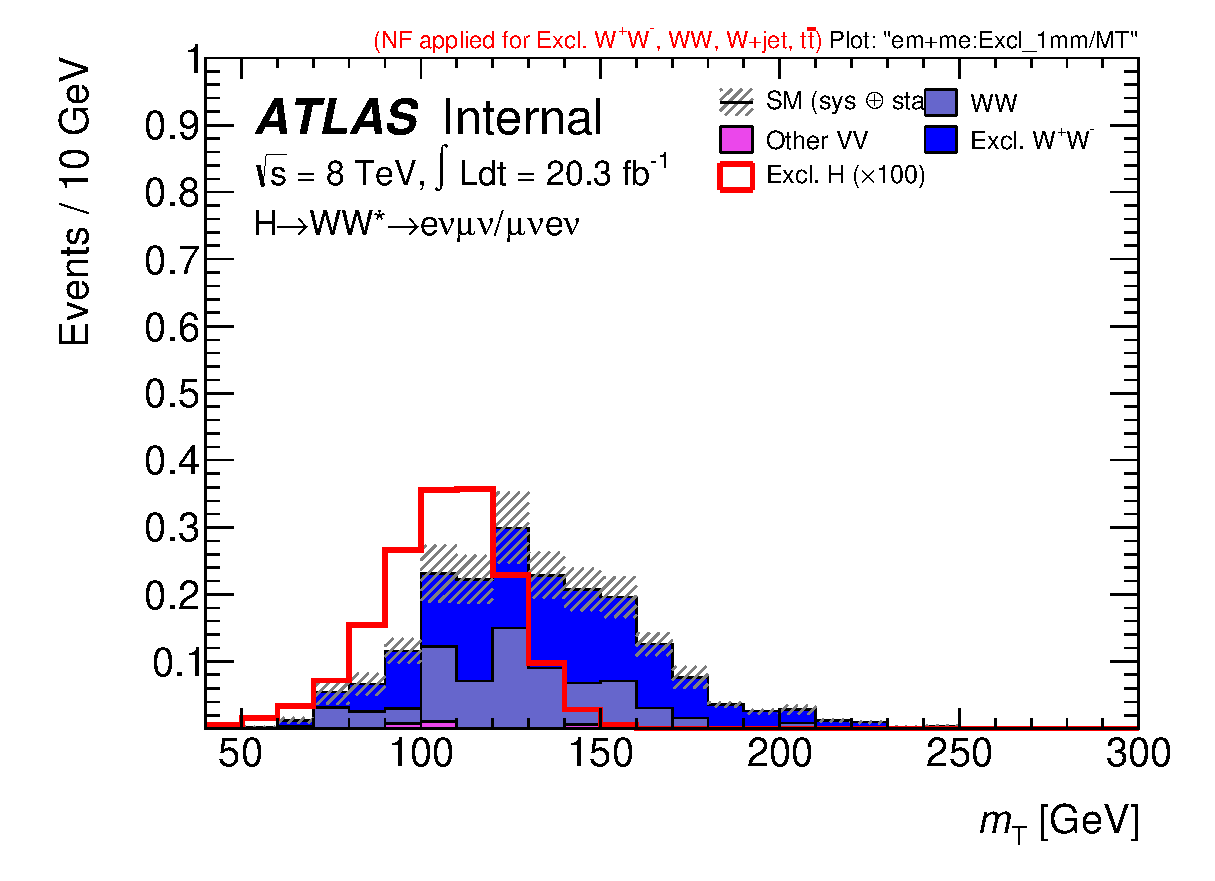
\includegraphics[width=\linewidth]{emme_Excl_1mm_MT_mh125_lin.eps}
\caption{\mt\ for events expected in the signal region. The major backgrounds
expected are exclusive and inclusive WW.}
\label{fig:results}
\end{figure}

\par An expected limit on the exclusive Higgs cross section was computed from these results. The only 
systematic uncertainty included in the calculation was on the integrated luminosity. The result of the 
fit is therefore statistical. Systematic uncertainties are currently being evaluated and the expected 
limit is under constant modification. Table~\ref{table:limits} shows the current results of the limit 
on the exclusive higgs cross section with the branching ratio factored in. This corresponds to a limit 
on the total production cross-section of 770 fb on the exclusive higgs. Compare this value with 3 fb 
predicted by the KMR model.   

\begin{table}[!h]
\begin{center}
\begin{tabular}{cc|cccc}
Cut & Limit [pb] & $+1\sigma$ & $+2\sigma$ & $-1\sigma$ & $-2\sigma$ \\
\hline
1 mm & 0.010 & 0.015 & 0.024 & 0.007 & 0.006 \\
\end{tabular}
\end{center}
\caption{Limits set on $\sigma\times BR (H\rightarrow WW\rightarrow l\nu l\nu) [pb]$ \@ 95\% CL 
using a 1-bin fit on \mt. The only systematic uncertainty considered is from integrated luminosity.}
\label{table:limits}
\end{table}
